\section{Experimental Results}

\subsection{RQ1: Targeted Elements}
\label{sec:hpath-results-rq1}

\begin{figure}
\centering
\subfloat[Targeted by GUI-based tests]{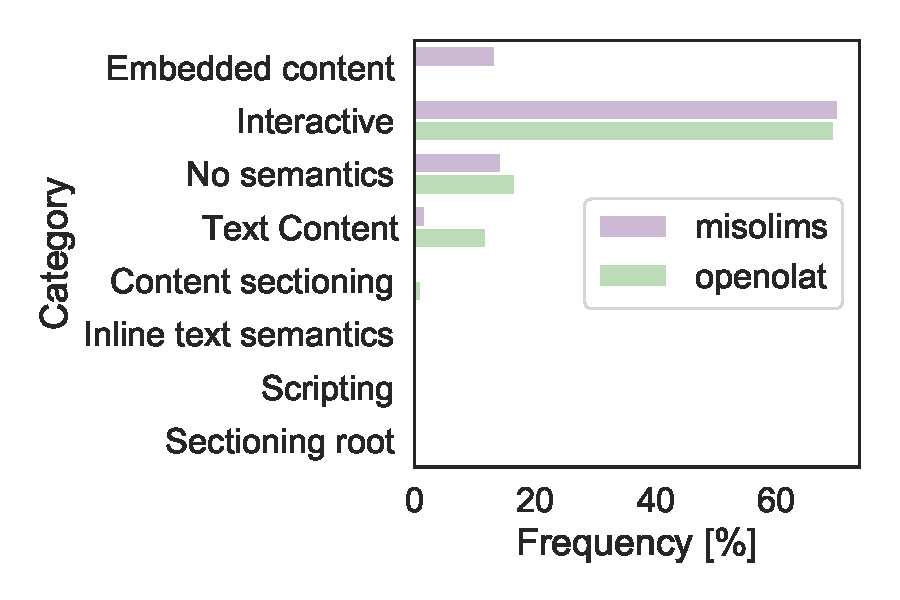
\includegraphics[width=0.45\textwidth]{figures/hpath/category-target-frequency.pdf}\label{fig:hpath-results-frequency-target}}
\subfloat[Present in DOM]{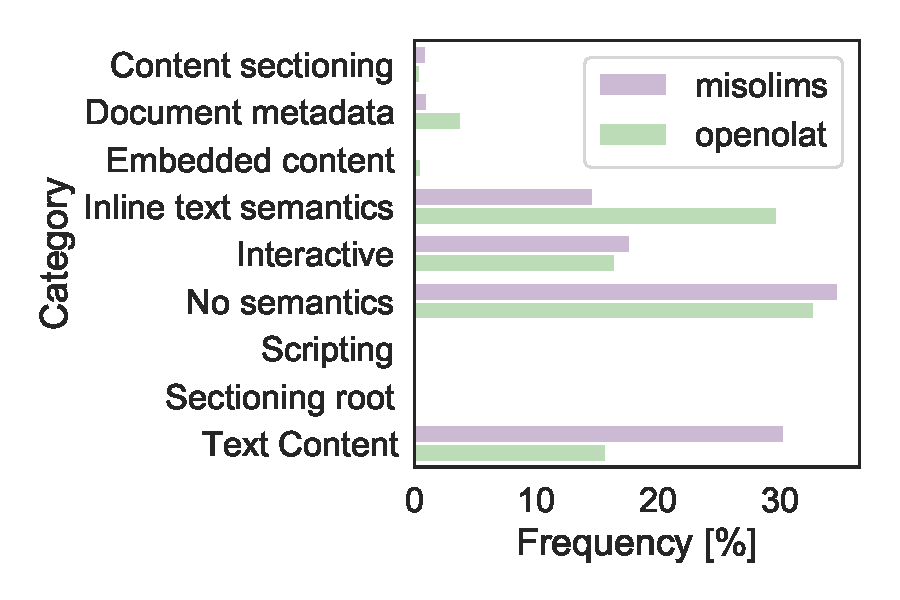
\includegraphics[width=0.45\textwidth]{figures/hpath/category-dom-frequency.pdf}\label{fig:hpath-results-frequency-dom}}
\caption{Percentages of elements (a) targeted by GUI-based tests and (b) present in the DOM for MISO LIMS and OpenOLAT across all versions aggregated by category.}  
\label{fig:hpath-results-frequency}
\end{figure}

In this RQ we evaluate the prevalence of each type of element targeted by GUI-based tests. Indeed, HPath makes strong assumptions about the type of elements being targeted by tests. For instance, elements from the Inline Text Semantics category and elements with no semantic attached ($E_{div}$ and $E_{span}$) that are not rendered cannot be reached by our approach. Furthermore, two (\emph{label} and \emph{text}) out of the four predicates present in the current implementation specifically target elements of the Interactive category. The institution behind these assumptions is that GUI-based tests interact with the application in the same fashion as a user would, through visible GUI components. 

Figure~\ref{fig:hpath-results-frequency} presents the distribution of target elements grouped by their semantic categories. It contrasts the frequency of elements targeted by GUI-based tests (Figure~\ref{fig:hpath-results-frequency-target}) to their overall frequency in the HTML document (Figure~\ref{fig:hpath-results-frequency-dom}). The discrepancy between the two shows that not all elements are of interest to testers. Indeed, the most prevalent categories in the HTML documents are No Semantics with 34.77\% and 32.82\% for MISO LIMS and OpenOLAT respectively, Inline Text Semantics with 29.76\% for OpenOLAT and Text Content with 30.32\% for MISO LIMS. However, Figure~\ref{fig:hpath-results-frequency-target} shows a very different picture, where the overwhelming category is Interactive with 70.27\% and 69.70\% for MISO LIMS and OpenOLAT respectively, confirming our hypothesis.

However, looking at Figure~\ref{fig:hpath-results-frequency-target} we observe a non-negligible amount of elements with no semantics accounting for 14.45\% in MISO LIMS and 16.71\% in OpenOLAT. After reviewing the tests it appears that some assertions and synchronization points target portions of the DOM defined by a $e_{div}$. Therefore, while they do not hold any intrinsic semantic in the HTML standard they do act as an anchor point that can be targeted by test scripts to assess the presence of an underlying group of elements. A more detailed discussion is presented in Section~\ref{sec:hpath-results-rq2} regarding the impact on HPath.

Finally, two categories vary from one project to the other, namely, Embedded content and Text content. The presence of elements from the Embedded content in MISO LIMS (13.41\%) is explained by clickable images under an anchor element, thus behaving like Interactive Elements. As for the elements from Text Content category present in OpenOLAT (11.91\%), they are used when asserting that the SUT is in the expected state, thus, following our hypothesis.

To conclude this research question, we see that GUI-based tests typically target specific portions of the HTML document, namely, Interactive elements and visible components on the page (text and images). HPath, relies on relevant properties to specify these elements and offers good predicates when locating them. However, the proportion of target elements with no HTML semantic is not negligible, which could make HPath enable to locate these elements if they are not rendered on the screen. We investigate this possibility in the next research question. 

\subsection{RQ2: Element Properties Used by Locators}
\label{sec:hpath-results-rq2}

This RQ investigates the relative performance in exploiting properties of target elements in the location path. HPath, absolute XPath and Robula+ formulating different hypotheses on which properties of an element can be used to locate it, we compare the three approaches.

Before being able to analyze which properties of the DOM HPath can leverage, we need to ensure that the target elements are reachable by the technique. Indeed, as shown in Section~\ref{sec:hpath-results-rq1} around 15\% of the target elements might not be rendered on the page. It appears that HPath fails to retrieve the locator in 11.58\% of the cases for MISO LIMS and in 10.48\% for OpenOLAT. These target elements not being rendered on the page, HPath is enabled to retrieve them. When observing the data, we see that assertions and synchronization points can target $e_{div}$ to verify the presence of the underlying group of elements. However, in many cases, other elements could have been selected to yield the same result had the initial test automation engineer relied on HPath. For example, in the project OpenOLAT, a test waits for a calendar widget to be rendered on a page, thus waits for the containing $e_{div}$ identified by its id (fc-view-container). The widget offering a series of named buttons (monat, tag, jhar) the test could rely on those to assess the availability of the widget. In the remaining of the discussion, only elements reachable by HPath are considered.

\begin{figure}
\centering
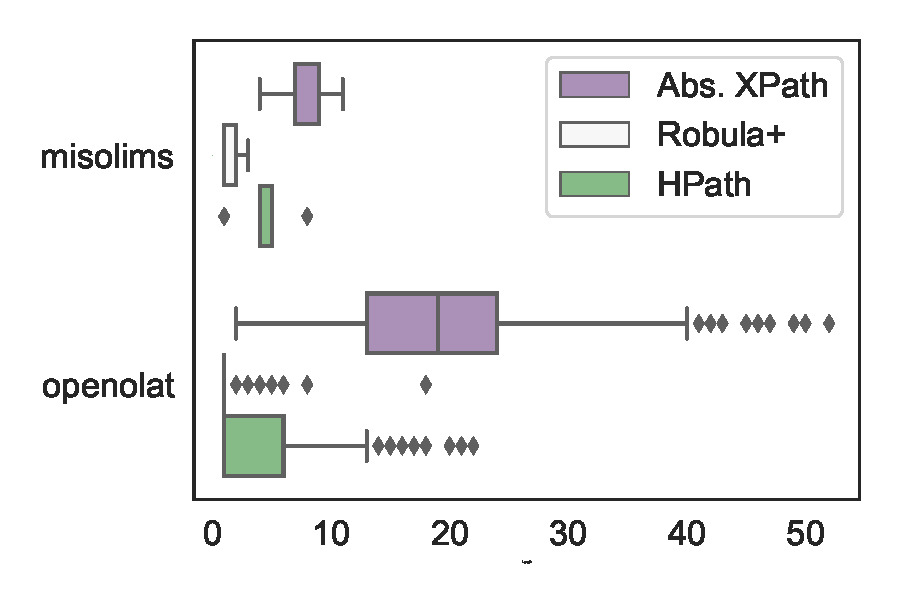
\includegraphics[width=0.6\columnwidth]{figures/hpath/canonical-selector-complexity-dist.pdf}
\caption{Length of absolute XPath, HPath and Robula+ for MISO LIMS and OpenOLAT across all versions.}  
\label{fig:hpath-results-lengths}
\end{figure}

We can now start our discussion on the properties by analyzing how much of the tree hierarchy is leaked when generating the location path. Figure~\ref{fig:hpath-results-lengths} displays the distribution of the length of the locators for the three strategies: absolute XPath, $L_{AXPath}$, Robula+ $L_{Robula+}$, and HPath, $L_{HPath}$. The figure shows a similar trend in both projects where absolute XPath yields the longest location paths with an average length of 8.6 and 18.7, Robula+ the shortest location path, with 1.6 and 1.0 and HPath lies between the two with 4.4 and 3.1, for MISO LIMS and OpenOLAT respectively. The lower performances of absolute XPath are to be expected since if no optimization can be done, both Robula+ and HPath generate a location path that is equal to the absolute XPath. Therefore $L_{HPath} \leq L_{AXPath}$ and $L_{Robula+} \leq L_{AXPath}$.

We compare the different distributions $L_{AXPath}$, $L_{Robula+}$ and $L_{HPath}$ using statistical Wilcoxon signed-rank test\footnote{Shapiro-Wilk test ($\alpha=0.001$) shows the non-normality of the distribution} ($\alpha=0.001$). The goal of this test is to assess whether or not there exists a statistical difference between the pairwise distributions. The results show that there is indeed a difference between all distributions, hence, the different strategies yield locators with different lengths. Then, we compute the pairwise effect size to determine how often lengths from one distribution are greater than in the other. The results show that in all the cases, the size effect is close to 1, \emph{i.e.} all samples from one distribution are greater than in the other, with the exception of $L_{HPath}$ and $L_{Robula+}$ for the OpenOLAT project where the size effect is 0.68. This is due to the fact that in many cases (58.52\% for HPath and 97.72\% for Robula+) both strategies manage to generate a location path of size 1, \emph{i.e.} not leaking hierarchy details of the DOM.

To conclude this discussion on the length of the location paths, we can see that strategies relying on different properties yield locators with different lengths. Relying on element attributes generates the shortest location path in both approaches and HPath exhibits better performances for OpenOLAT than MISO LIMS, even though the tree is deeper (as shown by the length of the absolute XPath). This is a consequence of OpenOLAT using the HTML5 standard, where MISO LIMS implements HTML4, offering more opportunities for HPath to generate good predicates.

\begin{table}
\centering
\caption{Properties of the context element leveraged by HPath and Robula+ predicates. \emph{Count} is the number of locators using a property as a predicate and \emph{\%} is the percentage among all the locators collected.}
\label{tab:hpath-results-properties}
\begin{tabular}{>{\raggedright}m{0.4in}>{\raggedright}m{0.5in}>{\raggedleft}m{0.4in} >{\raggedleft}m{0.4in}>{\raggedleft}m{0.5in} >{\raggedleft}m{0.4in}}
\toprule
\textbf{\scriptsize{Strategy}} & \textbf{\scriptsize{Property}} & \multicolumn{2}{c}{\textbf{\scriptsize{MISO LIMS}}} & \multicolumn{2}{c}{\textbf{\scriptsize{OpenOLAT}}}\tabularnewline
&   & \textbf{\scriptsize{Count}} & \textbf{\scriptsize{\%}} & \textbf{\scriptsize{Count}} & \textbf{\scriptsize{\%}}\tabularnewline
\toprule
\scriptsize{\textit{HPath}} & \scriptsize{\textit{caption}} & \scriptsize{0} & \scriptsize{0.00} & \scriptsize{0} & \scriptsize{0.00}\tabularnewline
& \scriptsize{\textit{figcaption}} & \scriptsize{0} & \scriptsize{0.00} & \scriptsize{0} & \scriptsize{0.00}\tabularnewline
& \scriptsize{\textit{label}} & \scriptsize{0} & \scriptsize{0.00} & \scriptsize{31,048} & \scriptsize{16.03}\tabularnewline
& \scriptsize{\textit{legend}} & \scriptsize{0} & \scriptsize{0.00} & \scriptsize{22,354} & \scriptsize{11.54}\tabularnewline
& \scriptsize{\textit{text}} & \scriptsize{227} & \scriptsize{1.64} & \scriptsize{93,031} & \scriptsize{48.02}\tabularnewline
& \scriptsize{\textit{\textbf{total}}} & \scriptsize{\textbf{227}} & \scriptsize{\textbf{1.64}} & \scriptsize{\textbf{142,103}} & \scriptsize{\textbf{73.35}}\tabularnewline
\hline
\scriptsize{\textit{Robula+}} & \scriptsize{\textit{id attr.}} & \scriptsize{5,161} & \scriptsize{32.93} & \scriptsize{143,334} & \scriptsize{66.23}\tabularnewline
& \scriptsize{\textit{class attr.}} & \scriptsize{412} & \scriptsize{2.63} & \scriptsize{48,483} & \scriptsize{22.40}\tabularnewline
& \scriptsize{\textit{name attr.}} & \scriptsize{207} & \scriptsize{1.32} & \scriptsize{150} & \scriptsize{0.07}\tabularnewline
& \scriptsize{\textit{title attr.}} & \scriptsize{0} & \scriptsize{0.00} & \scriptsize{3,094} & \scriptsize{1.43}\tabularnewline
& \scriptsize{\textit{text}} & \scriptsize{0} & \scriptsize{0.00} & \scriptsize{17751} & \scriptsize{8.20}\tabularnewline
& \scriptsize{\textit{\textbf{total}}} & \scriptsize{\textbf{5780}} & \scriptsize{\textbf{36.88}} & \scriptsize{\textbf{212558}} & \scriptsize{\textbf{99.80}}\tabularnewline
\bottomrule
\end{tabular}
\end{table}

Therefore, we conduct a fine-grained analysis to understand which properties HPath and Robula+ are able to leverage to compute the location path. Table~\ref{tab:hpath-results-properties} shows which element properties are exploited in the predicates of both approaches. Where HPath relies on properties from the HTML5 semantics, Robula+ exploits mainly attributes of the context element to generate the predicate.

Rows \emph{total} from Table~\ref{tab:hpath-results-properties} indicates how often a strategy is able to compute a predicate. We can see that in the case of OpenOLAT, both strategies often manage to compute predicate (73.35\% for HPath and 99.80\% for Robula+) but a lot less often in the case of MISO LIMS (1.64\% for HPath and 36.88\% for Robula+). Putting the results for MISO LIMS in contrast with the ones presented in Figure~\ref{fig:hpath-results-lengths}, we see that both strategies rely on other mechanisms to reduce the length. HPath relies on the rendering tree to prune $e_{div}$ that are not rendered. On the other hand, Robula+ during each refinement step evaluates the current location path to see if it uniquely identifies the target element. Doing so, it is able to take advantages of the fact that some element types are unique in the document, leading to location path such as "//img" in documents containing a single $e_{img}$ and manages to create a relative path 100\% of the time. However, relying on the uniqueness of an element type in a document can lead to locator breakages during SUT evolution, thus this strategy is not employed by HPath.

%we can see that in the case of MISO LIMS, the algorithm is almost never (1.64\%) capable of using a predicate while in the case of OpenOLAT, it is capable of relying on a predicate more than 70\% of the time. This drastic difference is explained by different factors. First, OpenOLAT uses HTML5 which has a much richer semantic that can be exploited by HPath while MISO LIMS uses the HTML4 standard. Further analysis showed that a lot of the interaction with MISO LIMS element are actually cells located in tables. Unfortunately, HPath does not yet support any predicate that allow to extract semantically element of a table. Finally, even though some semantic elements existed in HTML4, the developers of MISO LIMS do not rely on them and prefer the heavy use of $E_{div}$, lacking semantic. However, as shown in Figure~\ref{fig:automatic_length_distribution}, HPath is able to shorten the expressions by removing the non visible $e_{div}$ from the expression.

The next point of our discussion addresses the type of predicate used by HPath. As expected, in the case of MISO LIMS, all predicates targeting HTML5 semantic elements cannot be leveraged and only the label property is used. In the case of OpenOLAT, two types of predicates are never used: \emph{caption} and \emph{figcaption}. Analyzing the HTML documents, it appears that none of them contain elements $e_{caption}$ or $e_{figcaption}$. The three remaining predicates \emph{label}, \emph{legend} and \emph{text} are all related to forms ($E_{legend}$) and interactive elements ($E_{label}$ and $N_{text}$ child of Interactive element) and can be successfully used by the HPath predicate.

Robula+ on the other hands relies on the attributes of the element to compute the predicate. We see that almost all the elements of OpenOLAT offer at least one attribute that can be used (91.60\%). However, in 8.20\% of the cases, Robula+ relies on the text contained in the element. Note that the text extraction of Robula+ consists in retrieving the content the child $n_{text}$ of the context element where HPath is relying on the process described in Section~\ref{sec:hpath-hpath-text-extraction}.

In conclusion, results show that HPath is able to compute a location path in 90\% of the cases and when HTML5 semantics are available in the HTML document, HPath is able to successfully compute predicates for over 70\% of target elements. In the cases where no HTML5 semantic is available HPath is still able to reduce the length of the location path by relying on the rendering tree it computes. Nevertheless, relying on attributes properties shows better results, but we argue that those properties are less resistant to change in the SUT and investigate it in the next research question.

\subsection{RQ3: Locators Resilience to SUT Evolution}
\label{sec:locator_evolution_analysis_results}

This third research question evaluates the impact of changes in the SUT on DOM-based locators. Relying on the methodology described in Section~\ref{sec:hpath-protocol-breakage-detection} we present in Table~\ref{tab:locator_breakage} the percentage of locators breakage following SUT evolution. 

The results show that the two projects have very different profiles. Indeed, locator breakages depending on the type of the properties evolving in the SUT, they may vary from one development cycle to the next. However, note that the two projects are quite mature with over 15,000 commits in almost 10 years for OpenOLAT and over 4,200 commits in 9 years for MISO LIMS. This explains why no deep structural changes are observed over the periods we analyze as the low breakage count for absolute XPath suggests. Our goal being to spot iso-functional locator breakages, this stability ensures that when a breakage is observed, it is not due to a deep functional evolution of the page.

From Table~\ref{tab:locator_breakage}, for MISO LIMS, Robula+ has the lowest number of breakages (10) and closely followed by HPath (26). Figure~\ref{fig:changes_intersect_misolims} shows the intersection of elements for which the locators break. It shows that absolute XPath is a superset of Robula+ and HPath suggesting that they only break following a change in the DOM hierarchy. Furthermore, there is no overlap between Robula+ and HPath, meaning that relying on different properties make the locators resilient to different types of SUT evolution (supporting the results from \textcite{Leotta2015}).

On the other hand, the OpenOLAT project offers a very different picture. When constructing the HTML document to serve to the client, the backend of OpenOLAT automatically generates id, based on the version of the project, in order to ease communication with the database management system. HPath offers in this case the best resilience to change breaking only 0.49\% of the time. Contrarily, Robula+, relying on element attributes, offers very poor performance breaking in 64.99\% of the cases. Figure~\ref{fig:changes_intersect_misolims} shows that there exists an overlap between the different strategies but that in general they all react differently to changes.

\begin{table}
\centering
\caption{Locator breakages due to SUT evolution. \emph{Count} is the number of locators that broke because of a change and \emph{\%} is the percentage among all the pairs collected.}
\label{tab:locator_breakage}
\begin{tabular}{>{\raggedright}m{0.6in}>{\raggedleft}m{0.4in} >{\raggedleft}m{0.2in}>{\raggedleft}m{0.4in} >{\raggedleft}m{0.2in}}
\toprule
\textbf{\scriptsize{Strategy}} & \multicolumn{2}{c}{\textbf{\scriptsize{MISO LIMS}}} & \multicolumn{2}{c}{\textbf{\scriptsize{OpenOLAT}}}\tabularnewline
    & \textbf{\scriptsize{Count}} & \textbf{\scriptsize{\%}} & \textbf{\scriptsize{Count}} & \textbf{\scriptsize{\%}}\tabularnewline
\toprule
\scriptsize{\textit{Abs. XPath}} & \scriptsize{56} & \scriptsize{2.02} & \scriptsize{174} & \scriptsize{0.63}\tabularnewline
\scriptsize{\textit{Robula+}} & \scriptsize{10} & \scriptsize{0.36} & \scriptsize{17976} & \scriptsize{64.99}\tabularnewline
\scriptsize{\textit{HPath}} & \scriptsize{26} & \scriptsize{0.94} & \scriptsize{135} & \scriptsize{0.49}\tabularnewline
\bottomrule
\end{tabular}
\end{table}

\begin{figure}
\centering
\subfloat[MISO LIMS]{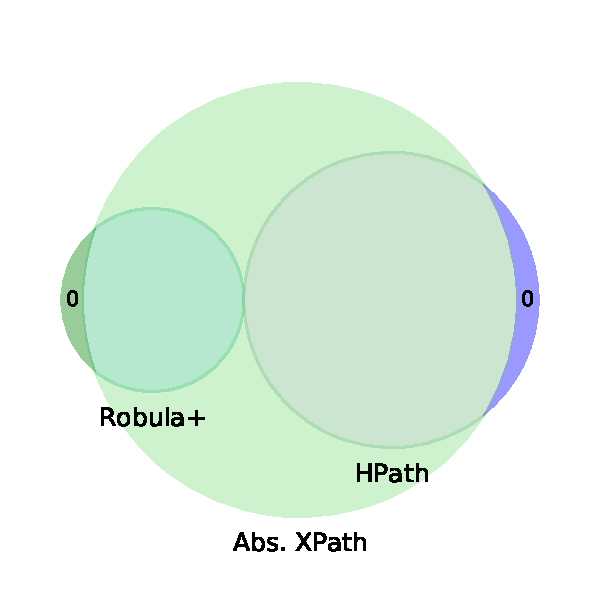
\includegraphics[width=0.45\columnwidth]{figures/hpath/changes-intersect-misolims.pdf}\label{fig:changes_intersect_misolims}}
\subfloat[OpenOLAT]{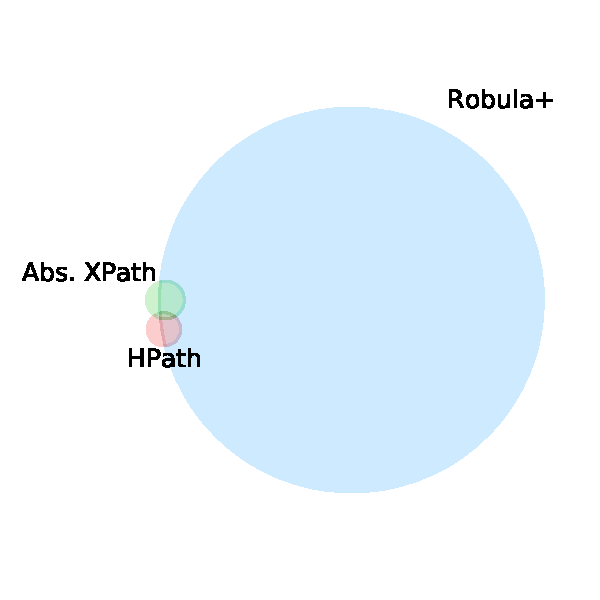
\includegraphics[width=0.45\columnwidth]{figures/hpath/changes-intersect-openolat.pdf}\label{fig:changes_intersect_openolat}}
\caption{Overlap of locators having breakage for Absolute XPath (green), Robula+ (blue) and HPath (red).}  
\label{fig:changes_intersect}
\end{figure}

To better understand which properties of the elements causes the locators to break, Table~\ref{tab:breakage_cause} shows the origin of the failure of the locator. To compute the origin, we compared the breaking location path from  $version_A$ to the passing one computed from $version_B$. The results of the fine-grained difference algorithm between the pair of locators point out the cause of the breakage. 

In the case of MISO LIMS, most of the failures happened in the position predicate, this related to the hierarchy structure of the DOM. Again, in the case of OpenOLAT, the profile is more diverse. Robula+ is not affected by changes in the element types (NameTest) in comparison to the other approaches, but is sensitive to attributes changes, leading to poor resilience to the evolution of the SUT where breakage due to the id contributed to 97.61\% of the breakage. Finally, when HPath is able to compute a predicate, it is resilient and never breaks in our dataset (Row \emph{Any Predicate} from Table~\ref{tab:breakage_cause}).  

\begin{table}
\centering
\caption{Properties causing locator breakages. \emph{Count} is the number of locators breaking because of a property and \emph{\%} is the percentage among all the breaking locators for that strategy.}
\label{tab:breakage_cause}
\begin{tabular}{>{\raggedright}m{0.6in}>{\raggedright}m{1.2in}>{\raggedleft}m{0.25in} >{\raggedleft}m{0.4in}>{\raggedleft}m{0.4in} >{\raggedleft}m{0.4in}}
\toprule
\textbf{\scriptsize{Strategy}} & \textbf{\scriptsize{Cause}} & \multicolumn{2}{c}{\textbf{\scriptsize{MISO LIMS}}} & \multicolumn{2}{c}{\textbf{\scriptsize{OpenOLAT}}}\tabularnewline
 &   & \textbf{\scriptsize{Count}} & \textbf{\scriptsize{\%}} & \textbf{\scriptsize{Count}} & \textbf{\scriptsize{\%}}\tabularnewline
\toprule
\scriptsize{\textit{Abs. XPath}} & \scriptsize{\textit{NameTest}} & \scriptsize{0} & \scriptsize{0.00} & \scriptsize{60} & \scriptsize{34.48}\tabularnewline
 & \scriptsize{\textit{Predicate position}} & \scriptsize{56} & \scriptsize{100.00} & \scriptsize{114} & \scriptsize{65.52}\tabularnewline
 \hline
\scriptsize{\textit{Robula+}} & \scriptsize{\textit{NameTest}} & \scriptsize{0} & \scriptsize{0} & \scriptsize{11} & \scriptsize{0.06}\tabularnewline
 & \scriptsize{\textit{Predicate position}} & \scriptsize{10} & \scriptsize{100.00} & \scriptsize{2} & \scriptsize{0.01}\tabularnewline
 & \scriptsize{\textit{Predicate id attr.}} & \scriptsize{0} & \scriptsize{0.00} & \scriptsize{17,578} & \scriptsize{97.79}\tabularnewline
 & \scriptsize{\textit{Predicate class attr.}} & \scriptsize{0} & \scriptsize{0.00} & \scriptsize{11} & \scriptsize{0.06}\tabularnewline
 & \scriptsize{\textit{Predicate title attr.}} & \scriptsize{0} & \scriptsize{0.00} & \scriptsize{77} & \scriptsize{0.43}\tabularnewline
 & \scriptsize{\textit{Predicate text content}} & \scriptsize{0} & \scriptsize{0.00} & \scriptsize{281} & \scriptsize{1.56}\tabularnewline
 \hline
\scriptsize{\textit{HPath}} & \scriptsize{\textit{NameTest}} & \scriptsize{0} & \scriptsize{0.00} & \scriptsize{119} & \scriptsize{88.14}\tabularnewline
 & \scriptsize{\textit{Predicate position}} & \scriptsize{26} & \scriptsize{100.00} & \scriptsize{16} & \scriptsize{11.85}\tabularnewline
 & \scriptsize{\textit{Any Predicate}} & \scriptsize{0} & \scriptsize{0.00} & \scriptsize{0} & \scriptsize{0.00}\tabularnewline
\bottomrule
\end{tabular}
\end{table}

In conclusion, when HPath can generate predicates they lead to robust and flexible locators. However, it can be hard for the approach to extract the necessary properties as shown in section~\ref{sec:locator_evolution_analysis_results}. Therefore, while the results are promising, more research needs to be conducted to better exploit the rendering properties present in the HTML5 semantics. Furthermore, better reliance on the standard by developers would improve the performances of tool relying on the semantic of the language.